\documentclass[12pt,          % font size: 11pt or 12pt
               ms,           % degree:    ms or phd
               doublespacing % spacing: onehalfspacing or doublespacing
               ]{ncsuthesis}

%%----------------------------------------------------------------------------%%
%%------------------------------ Import Packages -----------------------------%%
%%----------------------------------------------------------------------------%%

\usepackage{booktabs}  % professionally typeset tables
\usepackage{amsmath}
\usepackage{textcomp}  % better copyright sign, among other things
\usepackage{xcolor}
\usepackage{lipsum}    % filler text
\usepackage{subfig}    % composite figures
\usepackage[square, numbers]{natbib}
\usepackage{listings}
\usepackage{url}



%%----------------------------------------------------------------------------%%
%%---------------------------- Formatting Options ----------------------------%%
%%----------------------------------------------------------------------------%%
%%

%% -------------------------------------------------------------------------- %%
%% Disposition format -- any titles, headings, section titles
%%  These formatting commands affect all headings, titles, headings,
%%  so sizing commands should not be used here.
%%  Formatting options to consider are
%%     +  \sffamily - sans serif fonts.  Dispositions are often typeset in
%%                    sans serif, so this is a good option. 
%%     +  \rmfamily - serif fonts
%%     +  \bfseries - bold face
%\dispositionformat{\sffamily\bfseries}   % bold and sans serif
\dispositionformat{\bfseries}            % bold and serif

%% -------------------------------------------------------------------------- %%
%% Formatting for centered headings - Abstract, Dedication, etc. headings
%%  This is where one might put a sizing command.
%%  \MakeUppercase can be used to typeset all headings in uppercase.
\headingformat{\large\MakeUppercase}   % All letters uppercase
%\headingformat{\large}                % Not all uppercase
%\headingformat{\Large\scshape}        % Small Caps, used with serif fonts.

%% Typographers recommend using a normal inter-word space after
%% sentences. TeX's default is to add an wider space, but \frenchspacing
%% gives a normal spacing. Comment out the following line if you prefer
%% wider spaces between sentences.
\frenchspacing


%% -------------------------------------------------------------------------- %%
%%  Optional packages
%%    A number of compatible packages to improve the look and feel of
%%    your document are available in the file optional.tex 
%%    (For example, hyperlinks, fancy chapter headings, and fonts)
%% To use these options, uncomment the next line and see optional.tex
%%%  Optional Packages to consider.   These packages are compatible with
%%    ncsuthesis.  

%% -------------------------------------------------------------------------- %%
%% Fancy chapter headings
%%  available options: Sonny, Lenny, Glenn, Conny, Rejne, Bjarne
\usepackage[Sonny]{fncychap}

%%----------------------------------------------------------------------------%%
%% Hyperref package creates PDF metadata and hyperlinks in Table of Contents
%%  and citations.  Based on feedback from the NCSU thesis editor, 
%%  the links are not visually distinct from normal text (i.e. no change
%%  in color or extra boxes).
\usepackage[
  pdfauthor={John Mark Smith},
  pdftitle={The Title},
  pdfcreator={pdftex},
  pdfsubject={NC State ETD Thesis},
  pdfkeywords={keyword1, keyword2},
  colorlinks=true,
  linkcolor=black,
  citecolor=black,
  filecolor=black,
  urlcolor=black,
]{hyperref}


%% -------------------------------------------------------------------------- %%
%% Microtype - If you use pdfTeX to compile your thesis, you can use
%%              the microtype package to access advanced typographic
%%              features.  By default, using the microtype package enables
%%              character protrusion (placing glyphs a hair past the right 
%%              margin to make a visually straighter edge)
%%              and font expansion (adjusting font width slightly to get 
%%              more favorable justification).
%%              Using microtype should decrease the number of lines
%%              ending in hyphens.
\usepackage{microtype}


%%----------------------------------------------------------------------------%%
%% Fonts 

%% ETD guidelines don't specify the font.  You can enable the fonts
%%  by uncommenting the appropriate lines.  Using the default Computer 
%%  Modern fonts is *not* required.  A few common choices are below.
%%  See http://www.tug.dk/FontCatalogue/ for more options.

%% Serif Fonts -------------------------------------------------
%%  The four serif fonts listed here (Utopia, Palatino, Kerkis,
%%  and Times) all have math support.


%% Utopia
\usepackage[T1]{fontenc}
\usepackage[adobe-utopia]{mathdesign}

%% Palatino
%\usepackage[T1]{fontenc}
%\usepackage[sc]{mathpazo}
%\linespread{1.05}

%% Kerkis
%\usepackage[T1]{fontenc}
%\usepackage{kmath,kerkis}

%% Times
%\usepackage[T1]{fontenc}
%\usepackage{mathptmx}


%% Sans serif fonts -------------------------

%\usepackage[scaled]{helvet}  % Helvetica
%\usepackage[scaled]{berasans} % Bera Sans



%%----------------------------------------------------------------------------%%
%%---------------------------- Content Options -------------------------------%%
%%----------------------------------------------------------------------------%%
%% Size of committee: 3, 4, 5, or 6 -- this number includes the chair
\committeesize{3}

%% Members of committee
%%  Each of the following member commands takes an optional argument
%%   to specify their role on the committee.
%%  For co-chairs, use the commands:
%%      \cochairI{Doug Dodd}
%%      \cochairII{Chris Cox}
%%
\chair{Dr. Robert St. Amant}
\memberI{Dr. Edward F. Gehringer}
\memberII{Dr. Christopher G. Healey}


%% Student writing thesis, \student{First Middle}{Last}
\student{Shishir Mahesh}{Kakaraddi} % a full middle name
%\student{John M.}{Smith} % a middle initial

%% Degree program
\program{Computer Science}

%% Thesis Title
%%  Keep in mind, according to ETD guidelines:
%%    +  Capitalize first letter of important words.
%%    +  Use inverted pyramid shape if title spans more than one line.
%%
%%  Note: To break the title onto multiple lines, use \break instead of \\.
\thesistitle{A Comparison of Summarization Techniques for Small Sets of Micro Blogs}

%% Degree year.  Necessary if your degree year doesn't equal the current year.
%\degreeyear{1995}


%%----------------------------------------------------------------------------%%
%%---------------------------- Personal Macros -------------------------------%%
%%----------------------------------------------------------------------------%%

%% A central location to add your favorite macros.

%% A few examples to get you started.
\newcommand{\uv}[1]{\ensuremath{\mathbf{\hat{#1}}}}
\newcommand{\bo}{\ensuremath{\boldsymbol{\Omega}}}
\newcommand{\eref}[1]{Eq.~\ref{#1}}
\newcommand{\fref}[1]{Figure~\ref{#1}}
\newcommand{\tref}[1]{Table~\ref{#1}}

%%---------------------------------------------------------------------------%%
\begin{document}

%%---------------------------------------------------------------------------%%
\frontmatter

%% ------------------------------ Abstract ---------------------------------- %%
\begin{abstract}

Microblogs are a popular way to keep abreast with important information about different topics. Half a billion people across the world use Twitter, and and 175 million tweets are posted each day. With so much available data, summarization is critical. This thesis examines the problem of summarizing tweets from a single Twitter user over the the course of a few weeks to a month, between 35 and 60 tweets. The summarization takes the form of a subset of those tweets. We have developed and compared algorithms that can be used to summarize tweets in this way. We describe an unsupervised algorithm that clusters tweets by topic, using information retrieval techniques, and then selects a specific tweet from each cluster, relying on sentiment. An experimental evaluation shows that this approach produces results that are not as good as those of human summarizers, but are better than an existing baseline for such summaries.

\end{abstract}


%% ---------------------------- Copyright page ------------------------------ %%
%% Comment the next line if you don't want the copyright page included.
\makecopyrightpage

%% -------------------------------- Title page ------------------------------ %%
\maketitlepage

%% -------------------------------- Dedication ------------------------------ %%
\begin{dedication}
\centering To my family, for their support, love  and encouragement\\
\centering To my advisor, Dr Robert St. Amant, for his guidance in research\\
\centering To all of my friends, for our friendships
\end{dedication}

%% -------------------------------- Biography ------------------------------- %%
\begin{biography}

Shishir Mahesh Kakaraddi was born on 21st July, 1987 in Belgaum, Karnataka, India. He received a Bachelor of Engineering degree in Information Science from M S Ramaiah Institute of Technology, Bangalore, India. He worked at IBM India Pvt Ltd as Software Developer for11 months and then he joined North Carolina State University to pursue his Masters degree in the Department of Computer Science. After completion of his Masters degree he will be joining VMware in Palo Alto, California as a Member of Technical Staff.

\end{biography}

%% ----------------------------- Acknowledgements --------------------------- %%
\begin{acknowledgements}

I would like to thank my advisor Dr. Robert St. Amant who provided his professional advice on research ideas and dissertation writing. I also want to thank other committee members, Dr.Edward Gehringer and Dr. Christopher Healey,  for spending their time reading my  and contributing valuable comments and suggestions.Thanks to Dr. Tessa Lau, Research Staff Member, IBM Research for motivating me to do research and for introducing me to my advisor. I want to thank my friends Sridevi Venugopal and Thothathri Srinivasan for providing their opinions on several intermediate results. I would like to thank Sina Bahram, Srinath Ravindran and others in the Knowledge Discovery Lab for their suggestions. I would also like to thank everybody who helped me with the evaluation of my research.

\end{acknowledgements}


\thesistableofcontents

\thesislistoftables

\thesislistoffigures


%%---------------------------------------------------------------------------%%
\mainmatter

\chapter{Introduction}
\label{chap-one}
Let's start with a few paragraph basics, here is how to make \textbf{bold}, 
and \textit{italics}, and \emph{emphasized}.  Let's say you need to cite 
something in your references, simply type \verb^\cite{key}^, which produces
\cite{einstein1935particle}.  
Some other references are \cite{golub1996matrix} and 
\cite{larsen1974asymptotic}.
Some \LaTeX{} compilers 
require a second compilation for citations and references 
to be sorted and matched properly in the resulting document.  

Here is a quotation:
\begin{quotation}
Alice, Bob and Carol are boring.  Who would even want to know their secret?
\end{quotation}

Let's say we need to make a list, try this on for size
\begin{enumerate}
  \item NCSU is great
  \item I like NCSU
  \item I really hope I can find a job when I graduate!
\end{enumerate} 

\section{Math enviroments}
\subsection{Equations}

There are many different ways to write equations, for example we could put 
$a^2 + b^2 = c^2$ directly into a sentence.  Or we could use the equation 
enviroment and do 
%
\begin{equation}
  a^2+b^2=c^2.
  \label{eq:one}
\end{equation} 
And from here we can later reference it by simply doing typing 
\verb^\ref{label}^, which gives \ref{eq:one}.  However, defining and using
equation and figure reference macros will ensure that the equation
references are consistent, instead of having Eq.~(1), Equation 3, Eqn 4
scattered through the thesis.  This template file defines \verb^\eref^
and \verb^\fref^ for this purpose. You can modify the macros to your liking
in the \texttt{YourName-thesis.tex} file.
For example, the command \verb^\eref{label}^ gives \eref{eq:one}.


If you don't need to reference an equation you may simply do this 
\[
  a^2 + b^2 = c^2.
\]

For Greek letters you must go to the math enviroments, for example 
$\alpha$, $\beta$, and $\gamma$.  Let's look at equations that cover 
multiple lines, none of these equations may be true or mean anything, but so 
that the reader can get some ideas.  In addition I will use some other useful 
notations like subscripts, superscripts, fractions, etc.  One important item 
of note is that one uses the ``ampersand" symbol to line up equations 
(also look at how I used quotations).
%
\begin{eqnarray}
\gamma_1 & = & \alpha^{\beta} + \psi_0 \frac{\psi_1}{\psi_2+\psi_3} \label{eq.two} \\
& = & \beta_1 + \beta_2 + \ldots + \beta_k \nonumber\\
& \rightarrow & E(\gamma_2) 
\end{eqnarray}

Alternatively, one can specify a slightly different enviroment if none of 
the equations need to be numbered.  Remember that if you are planning on 
referring to them later on, you must use a ``label" statement.
%
\begin{eqnarray*}
\gamma_1 & = & n^{-1/2} \displaystyle \sum_{i=1}^n \left[h(X_i,\beta_0)-E\{h(X_i,\beta_0)\}\right]\\
& \rightarrow & \hat q \pm \frac{\partial \gamma_2}{\partial \beta}. 
\end{eqnarray*}  
Lastly there may be times in which you want to use a non-italicized word 
your formula, such as an indicator function that may look like this 
$\mbox{I}\{\mu_i(1,\beta)>\mu_i(0,\beta)\}$ , if so just use the 
``mbox" statement.


You could use a multiline equation for long equations.  The environment
is \texttt{multline}.  Insert \verb^\\^ for line breaks.
\begin{multline*}
  \bo \cdot \vec{\nabla} \psi(\vec{r},\bo,E)
   + \Sigma_t(\vec{r},E)\psi(\vec{r},\bo,E) = \\
  \int_{4\pi} d\bo' \int_0^{\infty} dE' \, 
  \Sigma_s(\vec{r},\bo'\to\bo,E'\to E)\psi(\vec{r},\bo',E')
  + Q(\vec{r},\bo,E),
\end{multline*}
we operate with $\displaystyle\int_{0}^{\infty}\left(\,\cdot\,\right) dE$
to obtain
\begin{multline*}
  \bo \cdot \vec{\nabla} \tilde{\psi}(\vec{r},\bo)
  + \Sigma_t(\vec{r})\tilde{\psi}(\vec{r},\bo) = \\
  \int_{4\pi} d\bo' \int_0^{\infty} dE' \, \psi(\vec{r},\bo',E')
  \left [ \int_{0}^{\infty} dE \, \Sigma_s(\vec{r},\bo'\to\bo,E'\to E)
  \right ] + \tilde{Q}(\vec{r},\bo),
\end{multline*}

\chapter{Related Work}
\label{chap-two}
There has been considerable amount of work in the area of micro blog mining. The different techniques and results are discussed in this chapter.

\section{Twitter Classification}
Twitter classification is used as the first step in many different twitter mining techniques. It is used as an intelligent data cleaning method to remove the unnecessary tweets from the initial twitter dataset. \citet{Sakaki:2010:EST:1772690.1772777} use classification as an intelligent filter in their technique of detecting the occurrence, time and location of earthquakes and typhoons by mining tweets. They provide a multi step process to obtain this information. Their first step is to classify the tweets into two classes tweets pertaining to real earthquakes and tweets not pertaining to real earthquakes. They use a Support Vector Machine based classifier with different types of features like,

\begin{description}
\item[A.] Statistical Features (Number of words, Position of query word)
\item[B.] Keyword Features (Word vector of the Tweet)
\item[C.] Word Context Features (Words before and after the query word)
\end{description}

Their classifier does really well at detecting earthquake events when they use only statistical features. It has a F-value of 73.69\%. Its F-value is lower when they used other features 53.85\% and 57.14\% for B and C respectively. This is further emphasized by the work of \citet{Sriram:2010:STC:1835449.1835643}. They describe a technique for organizing tweets into different top level classes using a Naive Bayes classifier. The goal of their work is to classify sets of tweets into generic classes, such as News, Opinions, Deals, Events, or Private Messages. The best performing classifier relies on eight features, one nominal and the remaining binary, collectively called 8F:

\begin{enumerate}
\item author (nominal)
\item presence of shortening of words and slang terms,
\item time/event phrases,
\item opinion words,
\item emphasis words,
\item currency and percentage signs,
\item @username at the beginning of the tweet, and
\item @username within the tweet.
\end{enumerate}

The overall accuracy of 8F is around 95\%. Because the model uses author information, however, it will tend to be tuned to each user's tweeting habits. This is the main drawback of this approach; as such a trained model cannot be easily applied to tweets from new users. The authors write, "The author feature is found to be very discriminative in our dataset." They also test their work against a Bag-of-Words (BOW) feature set, and find that 8F improves performance by 32.1\% over BOW. So even they concluded that statistically computed features seem to perform significantly better than Bag of Words. Performance of the combined 7F+BOW (7F is 8F with the author feature removed) falls between 8F and BOW. 

\section{Twitter Summarization}
A substantial amount of work has been done in exploring different techniques to summarize tweets. The word summary has been used as a common term for any information that is concise and extracted from a larger body of tweets. It takes different structures based on the context. The techniques of extracting summary too differ significantly based on the context and application. \citet{DBLP:conf/icwsm/ChakrabartiP11} have described different approaches to summarize an American football game. They aim to recognize all the sub events in a game like touchdowns, field goals etc using the tweets pertaining to the game. They have evaluated three different algorithms for this task. The first algorithm is called SUMMALLTEXT based on calculating euclidean distance between word vectors of every pair of tweets and choosing the one with the least distance from all other tweets and highest distance from already chosen tweets. This process is repeated for a specified number of times. This approach has many drawbacks, It gives too much importance to the one major sub event, It cannot recognize two separate events of the same type like two touchdowns at different times. They take this as the baseline for evaluating their other algorithms. To differentiate the events better temporally they use an important parameter in summarizing a football game. They divide the tweets into different time slots and apply the SUMMALLTEXT. This results in temporally segregated set of sub events. This is called SUMMTIMEINT. It suffers mostly with the same problems as SUMMALLTEXT. Finally they describe a variant of Hidden Markov Model(HMM) which recognizes the changes in the language model over time better than the SUMMALLTEXT and SUMMTIMEINT. They call it SUMMHMM. They train the model for American football game before running the evaluation. The models generated are very specific to the type of event hence the model needs to be trained for every new type of event. The model mainly depends on bursts in tweet volume and changes in language model over time. This makes the model usable only for events which are like sports, where there are defined important moments which correlate to bursts in tweet volume. The evaluation shows that on an average recall is just 0.5 when top 30 tweets are extracted after the SUMMHMM computation. This shows that recognizing sub events is really a hard problem even when you consider trained models.

\citet{Nichols:2012:SSE:2166966.2166999} try to address the shortcomings of a trained model to recognize sub events and summarize them. To demonstrate their technique for summarizing sporting events they have used a running example of soccer. Apart from recognizing the sub events they aim to provide a set of sentences as summary of a soccer game. They use the burst in tweet volume information to detect  events like a goal, yellow card and penalty shoot etc. Each burst in tweet is considered a sub event they detect the exact burst of tweets and the collect all the tweets from start of the burst to the end of the tweet burst. This is considered as a cluster. They remove the noise and choose the top ‘n’ sentences from each cluster ranking them based on the phrase graph approach discussed in \citet{Sharifi:2010:SMA:1857999.1858099}. This model is unsupervised unlike other approaches used for summarizing tweets of an event. However this model relies on the fact that each burst of tweets is one event. This may not hold true if two important events occurred in quick succession. Quick succession of events in common in some sports like American football. \citet{DBLP:conf/icwsm/ChakrabartiP11} have reported that in their dataset of American football games 45\% of the interception-plays were followed by field-goals or touchdown-plays. They also cite this as a reason for some performance drop in there SUMMHMM approach.  \citet{Nichols:2012:SSE:2166966.2166999} have evaluated their model only on a soccer game which has relatively less number of events and generally the events for a soccer game are well spaced out in time compared to other games like American football or basketball. However their results show a recall ranging from 0.6 to 0.9 and a precision of around 0.9 for the soccer games they have evaluated. This is a promising result considering the difficulty of the problem.

Searching twitter for important real time information is an important application of twitter. Query phrase based summarization techniques have been explored for providing good search results. \citet{DBLP:conf/icwsm/OConnorKA10} have a built a system to summarize the search results for a given term from twitter. A user can enter a keyword, the output will be a clustered sets of tweets identifying the different subtopics about the keyword. They use a series of steps to identify these subtopics. They can be either unigrams, bigrams or trigrams. In the first step they tokenize and filter the words. In the next step they calculate the importance of each token using probability of occurrence in the result subset and general tweet corpus. Then they merge similar topics using jaccard coefficient of similarity between the n-grams. They remove near duplicate tweets by looking at trigrams. This approach is interesting and good to extract the sub topics from a given topic. However it relies heavily on the tokenizer and probability of occurrence of words. This can lead to non important but frequently used words being chosen as the topics in case of users' tweets. It is common for a particular user to use similar words over and over again which do not represent a sub topic. Example words like ‘president’, ’POTUS’ which stands for President of The United States etc are used extensively in President Barack Obama’s twitter feed. Using this algorithm they would get recognized as the main topics of clusters thus resulting in substandard results. 

A very well known approach to summarizing tweets based on query word is the technique described by \citet{Sharifi:2010:SMA:1857999.1858099}. They describe an algorithm called the Phrase Reinforcement(PR) algorithm which can be used summarize a set of tweets. They have described the algorithm as a method to filter search results for a query term on twitter. The PR algorithm begins by creating a phrase graph of all the tweets obtained with the query term as the root node. Then each phrase which occurs in the context of the root node is augmented to the phrase graph. Then the graph is weighted based on a scheme which weighs heavily on repetition of words. Then the sentence with the highest weight is taken out first and so on to generate a partial summary.  This technique could be used to summarize cluster of tweets which belong to a related event. However this technique is not suitable for summarizing cluster formed by tweets of a user because, we  found that same sets of words are not used adjacent to the topic phrase when we look at tweets of a single user. For example for a  topic like ‘health care’ which is seen as a topic in President Obama's tweets shows that the context is sometimes women's health and sometimes it is related to health insurance.


\chapter{Preliminary Development}
\label{chap-three}

There are different approaches to summarizing micro blogs.  Broadly we can divide the approaches into supervised and unsupervised learning approaches. The different approaches we explored are explained in this chapter. We describe the data collection and processing phases. Then we discuss the supervised classification technique. We try to classify tweets into representative and non representative tweets using generic statistical features. We discuss the result of these explorations below.  Then we look at unsupervised techniques like clustering using different algorithms and different features.

\section{Data Collection}
Twitter provides a very easy to access REST API for accessing a user’s tweets. It also provides REST API client bindings in many different languages. This makes collecting data from twitter easier compared to other micro blog services like Facebook etc. We collected data to conduct a  study in order to understand more about what people think are the representative tweets among a given set of tweets from a user. We built a website where users could enter twitter username of a person they follow. They will be shown the last 30 to 50 tweets of that person. Then the users can go through these tweets and choose what they think are the representative tweets. The website was a Ruby on Rails application which used Redis key value store as the data store. The data collection application could make calls to twitter API and get the latest tweets by a particular twitter user. We did this study on a total of 13 users. This initial study helps us understand how users choose summaries from a given set of tweets. When we put together the numbers in all 541 tweets were seen amongst the 13 users. They have chosen a total of 63 tweets from these as representative tweets.

\section{Data Preparation}
The tweets collected in the data collection phase have to be pre-processed and “cleaned” before they can be utilized to compute features.  In this phase, the tweets are pre-processed using the two techniques of “Stemming” and “Stopword Removal”. Stemming is a process where different forms of the word are reduced to its original root form. In our study, a standard porter stemmer has been used on all the words of the tweets for stemming them . They are then converted to lowercase words. Stopword Removal is a technique where commonly used english words which do not distinguish the sentence from others are removed. In this study, a stop word list in English is used to remove commonly used words in tweets like prepositions, conjunction. This process ensures that all our tweets-data now have only important words eliminating  the superfluous  words that are seen in all tweets but act as noisy data in our study. The stop word list used in our study is provided as an attachment in the appendix section of this document. The tweet data is now pre-processed and cleaned of noisy and irrelevant words and is ready to be processed. 

\section{Data Processing}
We use the dataset of 541 tweets as the dataset to conduct our exploration. We have seen that statistical features have been really good at classifying tweets. Using only statistical features would make the model very generic. This will allow us to use it on different datasets. We calculated the different statistical features which can be used to classify tweets as representative tweets and non representative tweets. These statistical features include Inverse Document Frequency(IDF) for each word of each tweet. It is a commonly used statistical metric in information retrieval. It is helpful in indicating whether a word is unique to a small set of documents or it is common across all documents.We also compute Spelling correctness for each word of each tweet. Then we use aggregations of these values as the features for the dataset. The set of features we chose for classifying tweets include

\begin{enumerate}
\item Number of Words in the tweet
\item Average length of words in a tweet
\item Maximum Inverse Document Frequency (IDF)
\item Position of the word with the Maximum IDF
\item Average IDF of the tweets
\item Sum of IDF of all the words in the tweet
\item Spelling correctness percentage of  a tweet
\item Number of URL’s in the tweet
\item Number of Hashtags in the tweet
\end{enumerate}

\section{Classification}
We created a comma separated values(CSV) file with all the tweets and the computed features. We did not use any features like Username or Bag of words etc which would make the model very specific to the dataset under consideration. We used Weka to run different classification algorithms and noted down the F-Measure. The results are tabulated in table \ref{tab:one}


\begin{table}
\caption{Classification Performance}
\label{tab:one}
\begin{center}
\begin{tabular}{lccl}
\toprule
Algorithm & Precision & Recall & F-Measure\\
\midrule
Support Vector Machine & 1 & 0.036 & 0.07\\
Naive  Bayes  & 0.25 & 0.055 & 0.09\\
\bottomrule
\end{tabular}
\end{center}
\end{table}


The dataset had around 10\% of the tweets classified as representative and the rest as not representative. This created an imbalance in the dataset. Many other algorithms like Bayes Net and J48 decision trees had a F-Measure of 0 for Representative tweets. We tried to balance the dataset by sampling only 10\% of the tweets from the non representative set of tweets. This too didn't change the F-Measure much. 

\section{Clustering}
We could not achieve good performance using supervised learning techniques. Unsupervised techniques are very flexible. For an unsupervised technique we can use the words and properties of the words in a tweet as parameters, we tagged each word of each tweet with a "parts of speech" tag. We also assigned a real number indicating the sentiment value of each word. 

Our first approach was to use bag of words as the feature set for clustering. We applied Expectation Maximization(EM)\cite{Gupta:2010:DNC:1798337.1798433} and XMeans \cite{Pelleg:2000:XEK:645529.657808} algorithm on the feature set. Euclidean distance was used as the distance metric between two tweets. We found that clustering was broad and few clusters were created using these algorithms. Unrelated tweets also were clustered together. In order to solve these problems we realized we cannot use all the words in a tweet as features. We applied a filter on the features where only nouns and verbs were chosen to be part of the word vector. This helped in reducing the unrelated tweets being clustered together. However only few clusters were generated since the number of clusters generated in both XMeans and EM depends on maximum log likelihood estimation. This resulted in generating very few clusters as the log likelihood of many cluster did not turn out to be maximum in our case. As the few clusters generated were not sufficient, we have modified our approach. Examples of summaries formed using XMeans and EM clusters are provided in the Appendix A. For example when we applied these algorithms on 50 tweets of President Barack Obama we got only 3 clusters. 


\chapter{System Development}
\label{chap-four}

The process of extracting summary tweets from a small set of tweets involves three steps.

\begin{enumerate}
\item Access the micro blogs and compute different features of the data.
\item Group the tweets into clusters. 
\item Choose a summary tweet from each cluster
\end{enumerate}

In this chapter we discuss the approaches we have taken to complete all the three steps.

\section{Computing Features}

In this step all tweets are converted to word vectors of a fixed size. First we convert each tweet to lower case. Then stemming and stop word removal is done. This new form of the tweet is stored as a processed tweet. The processed tweet is used to compute the Inverse Document Frequency (IDF) of each word in the tweet. Each word of the tweet is also tagged with a parts of speech (POS) tagger. At the end of this step we have the processed form of a tweet, we have the IDF values and the POS tags for each word. The next step is to filter the words from the processed tweet, we filter out all the words which are not tagged as nouns or verbs. This helps in making sure only important words are used as candidates for topics. Then we sort them based on IDF. Lower IDF means the word has been used many times in set of tweets hence is a good candidate for clustering. The top n words from the sorted array are considered as the feature vector. The number n is specified by the algorithm. 

\section{Clustering Algorithm}

Each tweet is a feature vector also known as a point for the purposes of explaining the algorithm. The set of feature vectors is an input to the clustering algorithm. The clustering algorithm is a modified version of KMeans clustering algorithm. The KMeans clustering algorithm takes two inputs, number of clusters to be formed and the input points. It returns the clusters. We use KMeans as a part of modified KMeans. In the first iteration of the algorithm input set of feature vectors is split into two clusters. If clusters obtained have a size less than a threshold value then they are added to the final clusters list. If the size of the cluster is bigger than the threshold value then they are added back to the pool of points to be clustered. This way the threshold number for size of a cluster to be accepted as a final cluster acts as a way to control granularity of the cluster.  If i clusters are output in a certain iteration and all have a size greater than the threshold value then in the next iteration we try to split the points into i+1 clusters. This breaks a deadlock in the algorithm and keeps the iterations going till we split the points into granular clusters. An other way to break deadlock when too many words are similar between tweets is to add more detail by increasing the number of words considered for clustering in the feature vector. 

Modified Kmeans (MKmeans) has many advantages. The most important advantage in the context of summarizing tweets is that it gives the user a easy way to understand and control the granularity of the summary returned. The threshold size for a cluster can be controlled by the user as it easy to understand its function. If the threshold size of a cluster is inversely proportional to the number of tweets in the summary. This is because if the threshold is higher then there will be less clusters output by the algorithm there by reducing the number of clusters in the summary.

\lstset{ stepnumber=1, frame=single,basicstyle=\footnotesize,caption={Distance calculation between tweets},language={Ruby}}
\begin{lstlisting}
def distance_measure(fv1,fv2,params_length)
  fv1 = fv1[0..params_length-1]
  fv2 = fv2[0..params_length-1]
  temp = Hash.new
  for word in fv1
    temp[word] = true
  end
  matches = 0
  for word in fv2
    if temp[word] == true
      matches += 1
    end
  end
  return params_length - matches
end
\end{lstlisting}

The KMeans algorithm used in the Listing \ref{modified:kmeans} is not randomly initialized but chooses equally spaced points as its centers for the first iteration. This helps in getting consistent results. The KMeans algorithm uses a custom defined distance measure in our implementation. The distance between two feature vectors is calculated in a simple way. The distance function takes three inputs. The two feature vectors and parameter length. The third argument is used to decide how many words from the feature vector are considered for calculation of the distance. The output is the distance between the two feature vectors. This type of distance function ensures we can find distance between two feature vectors which have only nominal values easily.

\lstset{ stepnumber=1, frame=single,basicstyle=\footnotesize,caption={Modified KMeans Algorithm in Ruby},language={Ruby},label={modified:kmeans}}
\begin{lstlisting}
def MKmeans(all_points,first_split,params_length,threshold_cluster_size)
    i = first_split #Number of Clusters to split into
    while !all_points.empty? #While All Points is not Empty
      clusters = KMeans(all_points,i,params_length)
      flag = 0
      all_points = Array.new
      for cluster in clusters
        if cluster.size <= threshold_cluster_size
          final_clusters << cluster
          flag = 1
        else
          all_points += cluster.points
        end
      end
      if flag == 0
        i += 1
      else
        params_length += 1
      end
    end
end
\end{lstlisting}

\section{Cluster Summary}

Each cluster from the clustering process represents a topic. It is meaningful to choose one tweet from each cluster as the summary tweet. Collectively they will be representing the different topics from the input. We explored a few ways to choose one sentence from each cluster. We tried three approaches for this, The first approach was to choose the cluster center as the most representative tweet. This ensured that the words that describe the topic are included in the tweet. When we tried this out on few users we saw that clusters centers often tend to be tweets with small number of words. They dint provide much information apart from the topic itself. To solve this problem we chose to pick the tweet with the highest number of words. This was our second approach. We compared the results with users choices we saw that users often dint choose them as summary tweets. This led us to the final approach based on sentiment. We calculated sentiment of a tweet as the sum of absolute value of sentiment of each word in the tweet. Then we choose the tweet with the highest sentiment in the cluster. This correlated better with user choices of summary. 

This completes the system description. To summarize we calculate feature vector for each tweet based on the IDF and sentiment values of each word of the tweet. The feature vectors are clustered using a modified KMeans algorithm. Each cluster represents a granular topic. We choose a tweet from each cluster based on sentiment to form the summary tweets of the micro blog. 






\chapter{Evaluation}
\label{chap-five}
\newcommand{\ctheaders}[8]%
{\begin{tabular}{r|ccc||ccc|}
% Headers:
 \multicolumn{1}{r}{} & \multicolumn{3}{c}{#1}
      & \multicolumn{3}{c}{#2} \\ \cline{2-7}
% Row 1:
 #3 % \hspace{\cta}
      & \hspace{\cta} & #5 & \hspace{\cta}
      & \hspace{\cta} & #7 & \hspace{\cta}\ctstrut \\ \cline{2-7}
% Row 2:
 #4 % \hspace{\cta}
      & \hspace{\cta} & #6 & \hspace{\cta}
      & \hspace{\cta} & #8 & \hspace{\cta}\ctstrut \\ \cline{2-7}
\end{tabular}}

We have tried many approaches to summarize micro blogs. We also described a modified version of KMeans which can summarize tweets. We have evaluated the performance of our Modified KMeans algorithm against a published algorithm called SUMMALLTEXT\cite{DBLP:conf/icwsm/ChakrabartiP11}. We have built a web application which can interface with the different components needed to do the evaluation. We describe the evaluation application, the experiment and the results of the experiment in this section.

\section{Experiment Setup}
Evaluation application is a Ruby on Rails framework based application. It is connected to a Redis key value store as shown in the figure \ref{fig:evalapp1}, It acts as the data source for this application. Using a key value store like Redis provides a lot of flexibility when compared to regular relational databases. The application is designed to access tweets from three different sources, First source is directly through the Twitter API. The second data source is the Redis data store and the third data source is plain text files. Once a set of tweets are extracted from twitter they are stored in Redis too for future use. This reduces the time lag in fetching data, It also helps in serving the same set of tweets to different users for different opinions about summary. 

\begin{figure}[hbtp]
\centering
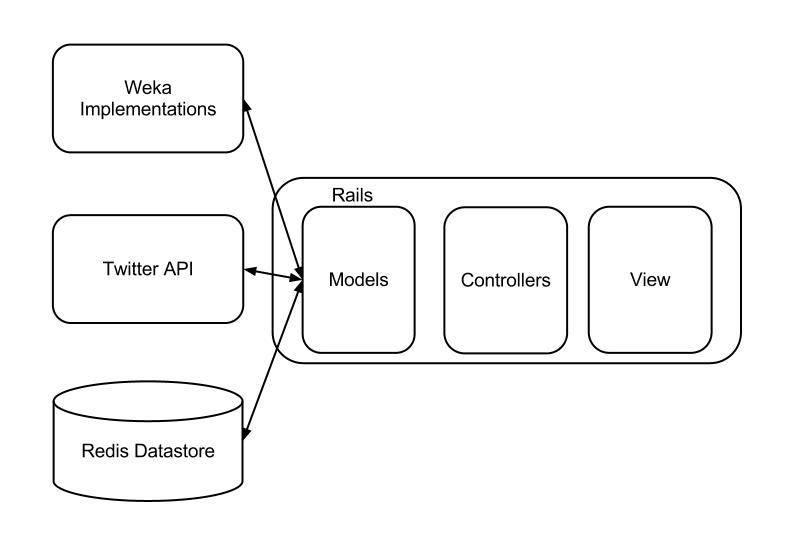
\includegraphics[width=0.9\textwidth]{Chapter-5/figs/evaluation_app_arch}
\caption{Highlevel Architecture of the Evaluation Application}
\label{fig:evalapp1}
\end{figure}

Stemming and Stopword removal was done using ruby libraries. We used a porter stemmer for stemming words. The list of stop words used for evaluation application is attached to the appendix. After stemming and stopword removal the processed tweet is formed. Then we used the ruby TF-IDF library to calculate the IDF of each word. We used the ruby bindings to the Stanford core natural language processing packages for parts of speech tagging. To compute other features we use other packages like spellchecker etc. 

The clustering algorithms are the central part of the evaluation application. We implemented two of the clustering algorithms SUMMALLTEXT and the Modified KMeans proposed by us. We wrote command line wrapper modules to Weka as shown in figure \ref{fig:evalapp1} This enables the application to make function calls to the Expectation Maximization and XMeans algorithms. The wrapper converts the features to a CSV file. Then it makes call to the appropriate algorithm using the command line and the CSV file as the input. It parses the results from a ARFF(Weka file format) file. Creates cluster objects and returns it to the Main program. The models and controllers of the Rails program make calls to the appropriate algorithms based on user preferences. The output is shown to the user on the web page. It can  also be written to a ARFF file, CSV file etc. 

We compared the Modified KMeans algorithm proposed by us against the SUMMALLTEXT algorithm in the evaluation. To choose a tweet from the cluster we used the sentiment based approach. With this setup we invited 12 users to take a test and rate the summaries generated by both the algorithms. Each user was asked to look at 35 - 60 tweets of a twitter user and choose representative tweets. In the next step they would look at the tweets chosen by them and the tweets chosen by one of the algorithms on the same screen. The screen also had a small form with three questions given below. 

\begin{enumerate}
\item Consider your summary as 5 out of 5. How much would you rate the summary generated by the computer
\item Consider the topic coverage of your summary to be 5 out of 5. How much would you rate the topic coverage of the summary generated by the computer
\item Provide comments about what should be added or removed
\end{enumerate}

Once the form is submitted the same screen would come up but this time the computer summary would be from another algorithm. The users are asked to rate this summary too. The order of appearance of algorithm results was shuffled. The users were also instructed ahead of time that it would be shuffled. Each user had to do the above evaluation for three different twitter profiles. Two of them were Barack Obama and Mitt Romney and the third one would be their choice. Several people looking at the same tweets and summarizing gives us a better understanding about how much the opinion varies. 

\section{Experiment Description}

We treat the three phases of the experiment as being independent.
Phase 1 involves the summarization of \#BarackObama tweets, Phase 2
the summarization of \#MittRomney tweets, and Phase 3 the
summarization of a participant-chosen set of tweets from different
Twitter users.

User ratings are discrete-valued data, which means that some common
types of summary and inferential statistics used for continuous data
are inappropriate.  We adopt the conventions of HCI research in
handling Likert scale data, using the median rather than the means as
a measure of central tendency, and using non-parametric tests for
comparisons.

Bar charts of the MKM and SAT summaries for each of the three
experiments are shown below.  The median of each distribution is shown
in Table~\ref{tab:modes}.

\section{Results}

\begin{table}
\begin{center}
\begin{tabular}{|l|llllll|llllll|}
\hline
& \multicolumn{3}{c}{MKM\slash G} & \multicolumn{3}{c|}{SAT\slash G} & \multicolumn{3}{|c}{MKM\slash T} & \multicolumn{3}{c|}{SAT\slash T} \\
\hline
Phase 1: \#BarackObama      & & 4    & & & 3.75 & & & 4 & & & 3.75 & \\
Phase 2: \#MittRomney       & & 4    & & & 3    & & & 4 & & & 3  & \\
Phase 3: (participant-chosen) & & 3.5  & & & 3    & & & 3.5 & & & 3  & \\
\hline
\end{tabular}
\end{center}
\caption{Medians}
\label{tab:modes}
\end{table}

The summaries in Table~\ref{tab:modes} suggest that MKM outperforms
SAT in each of the three phases.  We can go further by analyzing
the differences between the ratings of two summaries of a specific
Twitter user, per experiment participant.  

We use a Wilcoxon signed-rank test for comparing medians: MKM versus
SAT for the General condition, and MKM versus SAT for the Topic
condition.  The non-parametric Wilcoxon test is designed for
continuous data but is applied in practice to discrete ordinal data as
well.  The hypothesis we are testing is whether there is a significant
effect of Algorithm (MKM or SAT) on the medians of the distributions
in each condition, specifically whether MKM $>$ SAT.

For Phase 1, the \#BarackObama dataset, a Wilcoxon test shows no
significant effect of Algorithm in the General condition ($W = 12.0, p
= 0.12$), and similarly no significant effect in the General condition
($W = 11.0, p = 0.18$).

For Phase 2, the \#MittRomney dataset, a Wilcoxon test shows that
there is a significant effect of Algorithm in both the General
condition ($W = 27.5, p = 0.009$) and the Topic condition ($W = 25.5,
p = 0.01$).

For Phase 3, the dataset including participant-chosen Twitter users, a
Wilcoxon test shows that there is a significant effect of Algorithm in
both the General condition ($W = 20.0, p = 0.024$) and the Topic
condition ($W = 17.0, p = 0.008$).

Alternative tests, for which the user ratings are encoded in
categorical form, show comparable results.  

For example, we can reduce the rankings into three categories, in
which MKM $<$ SAT, MKM $=$ SAT, or MKM $>$ SAT.  A $\chi^2$ test can
then be used to test the hypothesis that the probability of MKM $<$
SAT is equal to the probability of MKM $>$ SAT.  This hypothesis is
rejected in all the same cases as above.
\chapter{Conclusion}
\label{chap-six}

In this chapter we discuss the features of modified KMeans algorithm. We discuss the advantages and disadvantages of the algorithm. We also discuss some of the improvements that are possible. There are many different opportunities to pursue in our work. We discuss about them in the future work section.

\section{Modified KMeans Discussion}

Modified KMeans algorithm provided better results in our study. It also provides easy to understand parameters which makes the algorithm interactive and customizable to to users needs. The algorithm has a worst case time complexity of $O(KN^{3})$ where $N^{3}$ comes from the KMeans calls and 'K' will be the number of clusters formed by the algorithm. This can be greatly reduced to almost just $N^{2}$ using memoization. We can reduce a lot of computations by storing the results of distance between all possible pairs of tweets. The distance function we provide can be used without trying to compute word vector each time as it uses nominal variables to compute the distance. However theoretically any other distance metric can be used too.

There are different customizations to the algorithm we havent explored yet. For example we have not tried a different distance algorithm. It would be good to see how this affects the output of the modified KMeans algorithm. We see that granularity increases if we decrease the threshold number of tweets in a cluster in our case. However we havent formally tested how the granularity changes with the threshold. The number of word to consider in the feature vector too depends on the length of the micro blog. We saw with experimentation that in our case starting with three words from the feature vector gives good results for tweets. Potentially it should be possible to use the same algorithm for more bigger blogs  too by changing the number of words to be considered to start with in the feature vector. We havent explored this part yet. 

In our evaluation we found that perception of granularity does change among users. We see from the comments provided by the users that some of them expected clusters with a single tweet also should be added. While others believed that the summary chosen by our algorithm too was elaborate. 

\section{Future Work}

All three steps of our system can be improved in different ways. The computation of features can be improved by adding more features like named entity recognition. This information could be useful when we try to choose words for the word vector and while finding distance between two vectors. We have used the dictionary approach for calculating sentiment for tweets. This approach is found to be better than using complex machine learning approaches according to \citet{DBLP:journals/corr/abs-0911-1583} for calculating sentiment. However since sentiment is so central to our approach it would be interesting to try other approaches to calculate sentiment. We could calculate the distance between words better than direct text matching if we used word net distance measures dicussed in [citation needed]. 

To make our clustering algorithm more precise, We could modify the algorithm to assign tweets to soft clusters. Then we could probably be able to recognize at what granularity the clusters become very similar. This impacts our assumption that each cluster groups tweets about a different topic. Since granularity can be controlled by the user this step would be necessary. 

Choosing a summary tweet from a cluster can be done in many ways. We tried to separate the tasks between the computer and the user in our approach. We found that it would be good to provide a set of summary tweets and assist the user to create a textual summary. There are techniques to create textual summary from similar sentences \cite{Barzilay:1999:IFC:1034678.1034760}. It would be interesting to explore that area too. 


%%---------------------------------------------------------------------------%%
%%  Bibliography 

%%  You can use the bibitem list.
%\bibliographystyle{unsrt}
%\begin{thebibliography}{99}
%\bibitem{cb02}
%Casella, G. and Berger, R.L. (2002)
%\newblock {\it Statistical Inference, Second Edition.}
%Duxbury Press, Belmont, CA.
%
%\bibitem{t06}
%Tsiatis, A.A. (2006)
%\newblock {\it Semiparametric Theory and Missing Data.}
%Springer, New York.
%
%\end{thebibliography}

%% or use BibTeX
\bibliography{YourName-thesis}{}
\bibliographystyle{plainnat}

%%---------------------------------------------------------------------------%%
% Appendices
\appendix
\chapter{Lorem Ipsum}

\section{A First Section}

\paragraph{Filler Text} \lipsum[1-6]
%
\begin{figure}
  \centering
  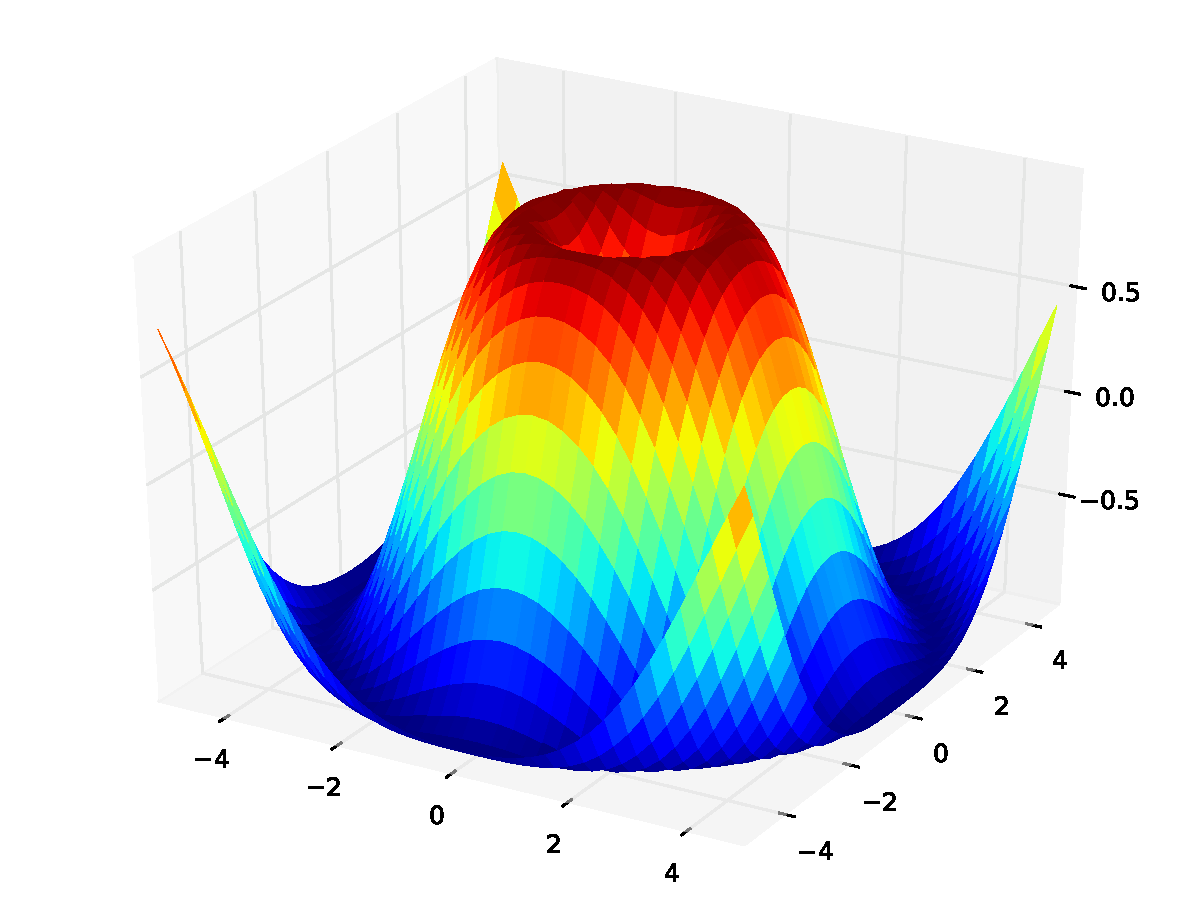
\includegraphics[width=0.6\textwidth]{Chapter-2/figs/threed}
  \caption{A figure in the appendix.}
  \label{fig:app}
\end{figure}
%
\lipsum[7-10]
\begin{table}
  \caption{A table in the appendix.}
  \label{tab:app}
  \begin{center}
    \begin{tabular}{lc}
      \toprule
      System & Author \\
      \midrule
      \TeX   & Donald Knuth   \\
      \LaTeX & Leslie Lamport \\
      \bottomrule
    \end{tabular}
  \end{center}
\end{table}
%

\section{A Second Section}

\lipsum[14-15]

\chapter{Stop Word List}
\label{chap:stopword}
"a" ,"able" ,"about" ,"above" ,"abst" ,"accordance" ,"according" ,"accordingly" ,"across" ,"act" ,"actually" ,"added" ,"adj" ,"adopted" ,"affected" ,"affecting" ,"affects" ,"after" ,"afterwards" ,"again" ,"against" ,"ah" ,"all" ,"almost" ,"alone" ,"along" ,"already" ,"also" ,"although" ,"always" ,"am" ,"among" ,"amongst" ,"an" ,"and" ,"announce" ,"another" ,"any" ,"anybody" ,"anyhow" ,"anymore" ,"anyone" ,"anything" ,"anyway" ,"anyways" ,"anywhere" ,"apparently" ,"approximately" ,"are" ,"aren" ,"arent" ,"arise" ,"around" ,"as" ,"aside" ,"ask" ,"asking" ,"at" ,"auth" ,"available" ,"away" ,"awfully" ,"b" ,"back" ,"be" ,"became" ,"because" ,"become" ,"becomes" ,"becoming" ,"been" ,"before" ,"beforehand" ,"begin" ,"beginning" ,"beginnings" ,"begins" ,"behind" ,"being" ,"believe" ,"below" ,"beside" ,"besides" ,"between" ,"beyond" ,"biol" ,"both" ,"brief" ,"briefly" ,"but" ,"by" ,"c" ,"ca" ,"came" ,"can" ,"cannot" ,"can't" ,"cause" ,"causes" ,"certain" ,"certainly" ,"co" ,"com" ,"come" ,"comes" ,"contain" ,"containing" ,"contains" ,"could" ,"couldnt" ,"d" ,"date" ,"did" ,"didn't" ,"different" ,"do" ,"does" ,"doesn't" ,"doing" ,"done" ,"don't" ,"down" ,"downwards" ,"due" ,"during" ,"e" ,"each" ,"ed" ,"edu" ,"effect" ,"eg" ,"eight" ,"eighty" ,"either" ,"else" ,"elsewhere" ,"end" ,"ending" ,"enough" ,"especially" ,"et" ,"et-al" ,"etc" ,"even" ,"ever" ,"every" ,"everybody" ,"everyone" ,"everything" ,"everywhere" ,"ex" ,"except" ,"f" ,"far" ,"few" ,"ff" ,"fifth" ,"first" ,"five" ,"fix" ,"followed" ,"following" ,"follows" ,"for" ,"former" ,"formerly" ,"forth" ,"found" ,"four" ,"from" ,"further" ,"furthermore" ,"g" ,"gave" ,"get" ,"gets" ,"getting" ,"give" ,"given" ,"gives" ,"giving" ,"go" ,"goes" ,"gone" ,"got" ,"gotten" ,"h" ,"had" ,"happens" ,"hardly" ,"has" ,"hasn't" ,"have" ,"haven't" ,"having" ,"he" ,"hed" ,"hence" ,"her" ,"here" ,"hereafter" ,"hereby" ,"herein" ,"heres" ,"hereupon" ,"hers" ,"herself" ,"hes" ,"hi" ,"hid" ,"him" ,"himself" ,"his" ,"hither" ,"home" ,"how" ,"howbeit" ,"however" ,"hundred" ,"i" ,"id" ,"ie" ,"if" ,"i'll" ,"im" ,"immediate" ,"immediately" ,"importance" ,"important" ,"in" ,"inc" ,"indeed" ,"index" ,"information" ,"instead" ,"into" ,"invention" ,"inward" ,"is" ,"isn't" ,"it" ,"itd" ,"it'll" ,"its" ,"itself" ,"i've" ,"j" ,"just" ,"k" ,"keep" ,"keeps" ,"kept" ,"keys" ,"kg" ,"km" ,"know" ,"known" ,"knows" ,"l" ,"largely" ,"last" ,"lately" ,"later" ,"latter" ,"latterly" ,"least" ,"less" ,"lest" ,"let" ,"lets" ,"like" ,"liked" ,"likely" ,"line" ,"little" ,"'ll" ,"look" ,"looking" ,"looks" ,"ltd" ,"m" ,"made" ,"mainly" ,"make" ,"makes" ,"many" ,"may" ,"maybe" ,"me" ,"mean" ,"means" ,"meantime" ,"meanwhile" ,"merely" ,"mg" ,"might" ,"million" ,"miss" ,"ml" ,"more" ,"moreover" ,"most" ,"mostly" ,"mr" ,"mrs" ,"much" ,"mug" ,"must" ,"my" ,"myself" ,"n" ,"na" ,"name" ,"namely" ,"nay" ,"nd" ,"near" ,"nearly" ,"necessarily" ,"necessary" ,"need" ,"needs" ,"neither" ,"never" ,"nevertheless" ,"new" ,"next" ,"nine" ,"ninety" ,"no" ,"nobody" ,"non" ,"none" ,"nonetheless" ,"noone" ,"nor" ,"normally" ,"nos" ,"not" ,"noted" ,"nothing" ,"now" ,"nowhere" ,"o" ,"obtain" ,"obtained" ,"obviously" ,"of" ,"off" ,"often" ,"oh" ,"ok" ,"okay" ,"old" ,"omitted" ,"on" ,"once" ,"one" ,"ones" ,"only" ,"onto" ,"or" ,"ord" ,"other" ,"others" ,"otherwise" ,"ought" ,"our" ,"ours" ,"ourselves" ,"out" ,"outside" ,"over" ,"overall" ,"owing" ,"own" ,"p" ,"page" ,"pages" ,"part" ,"particular" ,"particularly" ,"past" ,"per" ,"perhaps" ,"placed" ,"please" ,"plus" ,"poorly" ,"possible" ,"possibly" ,"potentially" ,"pp" ,"predominantly" ,"present" ,"previously" ,"primarily" ,"probably" ,"promptly" ,"proud" ,"provides" ,"put" ,"q" ,"que" ,"quickly" ,"quite" ,"qv" ,"r" ,"ran" ,"rather" ,"rd" ,"re" ,"readily" ,"really" ,"recent" ,"recently" ,"ref" ,"refs" ,"regarding" ,"regardless" ,"regards" ,"related" ,"relatively" ,"research" ,"respectively" ,"resulted" ,"resulting" ,"results" ,"right" ,"run" ,"s" ,"said" ,"same" ,"saw" ,"say" ,"saying" ,"says" ,"sec" ,"section" ,"see" ,"seeing" ,"seem" ,"seemed" ,"seeming" ,"seems" ,"seen" ,"self" ,"selves" ,"sent" ,"seven" ,"several" ,"shall" ,"she" ,"shed" ,"she'll" ,"shes" ,"should" ,"shouldn't" ,"show" ,"showed" ,"shown" ,"showns" ,"shows" ,"significant" ,"significantly" ,"similar" ,"similarly" ,"since" ,"six" ,"slightly" ,"so" ,"some" ,"somebody" ,"somehow" ,"someone" ,"somethan" ,"something" ,"sometime" ,"sometimes" ,"somewhat" ,"somewhere" ,"soon" ,"sorry" ,"specifically" ,"specified" ,"specify" ,"specifying" ,"state" ,"states" ,"still" ,"stop" ,"strongly" ,"sub" ,"substantially" ,"successfully" ,"such" ,"sufficiently" ,"suggest" ,"sup" ,"sure" ,"t" ,"take" ,"taken" ,"taking" ,"tell" ,"tends" ,"th" ,"than" ,"thank" ,"thanks" ,"thanx" ,"that" ,"that'll" ,"thats" ,"that've" ,"the" ,"their" ,"theirs" ,"them" ,"themselves" ,"then" ,"thence" ,"there" ,"thereafter" ,"thereby" ,"thered" ,"therefore" ,"therein" ,"there'll" ,"thereof" ,"therere" ,"theres" ,"thereto" ,"thereupon" ,"there've" ,"these" ,"they" ,"theyd" ,"they'll" ,"theyre" ,"they've" ,"think" ,"this" ,"those" ,"thou" ,"though" ,"thoughh" ,"thousand" ,"throug" ,"through" ,"throughout" ,"thru" ,"thus" ,"til" ,"tip" ,"to" ,"together" ,"too" ,"took" ,"toward" ,"towards" ,"tried" ,"tries" ,"truly" ,"try" ,"trying" ,"ts" ,"twice" ,"two" ,"u" ,"un" ,"under" ,"unfortunately" ,"unless" ,"unlike" ,"unlikely" ,"until" ,"unto" ,"up" ,"upon" ,"ups" ,"us" ,"use" ,"used" ,"useful" ,"usefully" ,"usefulness" ,"uses" ,"using" ,"usually" ,"v" ,"value" ,"various" ,"'ve" ,"very" ,"via" ,"viz" ,"vol" ,"vols" ,"vs" ,"w" ,"want" ,"wants" ,"was" ,"wasn't" ,"way" ,"we" ,"wed" ,"welcome" ,"we'll" ,"went" ,"were" ,"weren't" ,"we've" ,"what" ,"whatever" ,"what'll" ,"whats" ,"when" ,"whence" ,"whenever" ,"where" ,"whereafter" ,"whereas" ,"whereby" ,"wherein" ,"wheres" ,"whereupon" ,"wherever" ,"whether" ,"which" ,"while" ,"whim" ,"whither" ,"who" ,"whod" ,"whoever" ,"whole" ,"who'll" ,"whom" ,"whomever" ,"whos" ,"whose" ,"why" ,"widely" ,"willing" ,"wish" ,"with" ,"within" ,"without" ,"won't" ,"words" ,"world" ,"would" ,"wouldn't" ,"www" ,"x" ,"y" ,"yes" ,"yet" ,"you" ,"youd" ,"you'll" ,"your" ,"youre" ,"yours" ,"yourself" ,"yourselves" ,"you've" ,"z" ,"zero"





%%---------------------------------------------------------------------------%%
\backmatter


\end{document}
